% This file contains the text portion of the Documentation & Reporting portion of the project charter - Section 14

%%%%%%%%%%%%%%%%%%%%%%%%%%%%%%%%%%%%%%%%%%%%%%
%%%%%%% 14.1 DOCUMENTATION & REPORTING %%%%%%%
%%%%%%%%%%%%%%%%%%%%%%%%%%%%%%%%%%%%%%%%%%%%%%
% 14.1 MAJOR DOCUMENTATION DELIVERABLES
\subsection{Major Documentation Deliverables}

% 14.1.1 PROJECT CHARTER
\subsubsection{Project Charter}
The initial version of the Project Charter will be uploaded on October 3nd 2022. The final version of the Project charter will be uploaded on April 30th 2023. There is a possibility that the charter will be updated sprint to sprint as more information is received. Sections such as 14.2, 14.2.1, 14.2.5, etc, are most likely to be updated.

% 14.1.2 SYSTEM REQUIREMENTS SPECIFICATION
\subsubsection{Systems Requirements Specification}
The initial version of the SRS document will describe the features and behaviors of the Drone and the software we expect to utilize within the project. The initial version of the SRS document will be submitted on October 24, 2022. The final version of the SRS document will be submitted on April 30th, 2023 when the final version of the project charter will be submitted. Should changes occur after the initial version of the SRS document is submitted, we will update the appropriate document/s to reflect those changes.

% 14.1.3 ARCHITECTURAL DESIGN SPECIFICATION
\subsubsection{Architectural Design Specification}
November 14th, 2022 will be the deadline for the initial Architectural Design Specification (ADS). The final deadline for the ADS will be April 30th, 2022. Each team member can edit the ADS at any time, and all changes will be reflected for everyone on a shared Google Doc. In the process of developing the project, we will continue to update this shared document as needed.

% 14.1.4 DETAILED DESIGN SPECIFICATION
\subsubsection{Detailed Design Specification}
The initial version of the Detailed Design Specification (DDS) will reflect the state of hardware and software components at that time. If any changes are made to the hardware or software being utilized in the project after the initial version is submitted, then our team will update the DDS to reflect those changes. The initial version of the Detailed Design Specification will be submitted February 26th, 2023. The final version of the Detailed Design Specification will be submitted April 30th, 2023.

%%%%%%%%%%%%%%%%%%%%%%%%%%%%%%%%%%%%%%%%%%%%%%
%%%%%%%%% 14.2 RECURRING SPRINT ITEMS %%%%%%%%
%%%%%%%%%%%%%%%%%%%%%%%%%%%%%%%%%%%%%%%%%%%%%%
\subsection{Recurring Sprint Items}

% 14.2.1 PRODUCT BACKLOG
\subsubsection{Product Backlog}
As soon as the SRS is created, a backlog item will be created for each requirement. These items will be prioritized by necessity to get a test drone built, while also having working software. The handling of our team's backlog will be done by the Scrum Master. The team's backlog will be issued through a shared Google Sheet.

% 14.2.2 SPRINT PLANNING
\subsubsection{Sprint Planning}
There will be eight sprints throughout the duration of this project. Each of them would be planned taking into account lessons learned from previous sprints. The following methods will also be implemented:
\begin{itemize}
  \item Planning a sprint meeting after examining the team's availability
  \item Go over backlog and assigning ownership of tasks to team members
  \item Confirm new issues, impacts, and dependencies
  \item Reach a group consensus on time estimations
\end{itemize}

% 14.2.3 SPRINT GOAL
\subsubsection{Sprint Goal}
The sprint goal will be determined by the team during a meeting before the start of the sprint. The best way to keep the project stakeholders involved is by giving a report on our sprint goal to our sponsor on the first Friday of every sprint.

% 14.2.4 SPRINT BACKLOG
\subsubsection{Sprint Backlog}
The SCRUM master will be primarily in charge of managing which items are placed in the sprint backlog, and how much time is estimated for each of those tasks. An excel spreadsheet will be used to maintain our sprint backlog, update time estimates, and display a burndown chart.

% 14.2.5 TASK BREAKDOWN
\subsubsection{Task Breakdown}
Individual tasks will be first assigned by members who volunteer for that task. Time spent on tasks will be logged by each individual within the team on our Excel spreadsheet.

% 14.2.6 SPRINT BURN DOWN CHARTS
\subsubsection{Sprint Burn Down Charts}
When each team member logs their hours worked for each task in the Excel spreadsheet, there will be a Burn Down chart that gets updated automatically. The sprint spreadsheet will include specific sprint backlogs in which the general tasks for that sprint are divided into smaller parts. This will indicate which team member(s) worked on each subtask. The subtasks are not recorded per hour, yet. The total number of hours expended by each team member is included in a table for every sprint backlog.

\begin{figure}[h!]
    \centering
    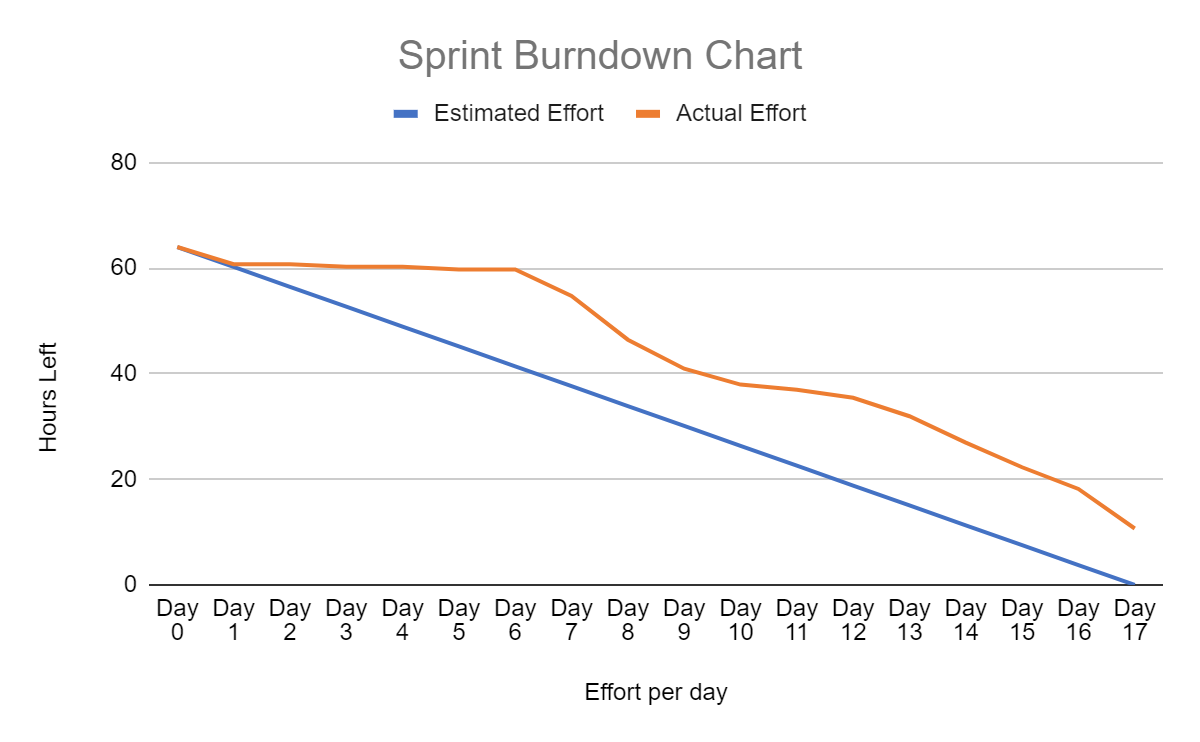
\includegraphics[width=1\textwidth]{images/burndown_example.png}
    \caption{Example sprint burn down chart}
\end{figure}

% 14.2.7 SPRINT RETROSPECTIVE
\subsubsection{Sprint Retrospective}
Following each sprint, the team will hold a retrospective meeting to discuss what went well and what could be improved. We will assign team tasks to each team member based on the sprint goals. Assigning tasks will keep team members accountable. Each task will be due at the end of each sprint.

% 14.2.8 INDIVIDUAL STATUS REPORTS
\subsubsection{Individual Status Reports}
Every week, there will be a Discord meeting to give a status report. Detailed information regarding a team member's goals, issues, and progress will be included in the team member's status reports.

% 14.2.9 ENGINEERING NOTEBOOKS
\subsubsection{Engineering Notebooks}
Software development team members are expected to update their engineering notebooks at the end of each sprint in order to hold each other accountable for their work. It is essential that each team member is able to communicate effectively regarding their engineering notebooks in order to hold one another accountable. A mid-sprint meeting can be used to discuss the targeted number of pages for the current sprint. To ensure quality control, the SCRUM master must sign off as a witness for each engineering notebook page.

%%%%%%%%%%%%%%%%%%%%%%%%%%%%%%%%%%%%%%%
%%%%%%% 14.3 CLOSEOUT MATERIALS %%%%%%% 
%%%%%%%%%%%%%%%%%%%%%%%%%%%%%%%%%%%%%%%
\subsection{Closeout Materials}

% 14.3.1 SYSTEM PROTOTYPE
\subsubsection{System Prototype}
In the final system prototype the drone will contain features that have been discussed in previous sections. To reiterate, the final system prototype will include the following: GPS and RTK, camera for IR blasting and QR code detection, a cube orange flight controller, and software that configures autonomous flight. There will be a Prototype Acceptance Test with the customer, they expect to see a prototype by the end of the fall 2022 semester. There will be off-site testing in the Maverick stadium as it is intended to be an outdoor competition if there are favorable weather conditions.

% 14.3.2 PROJECT POSTER
\subsubsection{Project Poster}
In addition to an architectural diagram, the poster will also explain Python use cases and describe the components of the drone.

% 14.3.3 WEB PAGE
%\subsubsection{Web Page}

% 14.3.4 DEMO VIDEO
\subsubsection{Demo Video}
As certain parts of the project become demonstrable, demo videos will be provided. Demo videos will demonstrate key aspects of the project and how they behave and respond in real-world environments. Videos will vary in length depending on what is being demonstrated.

% 14.3.5 SOURCE CODE
\subsubsection{Source Code}
Version control and source code maintenance will be handled by the team using Git and GitHub. The source code will not be accessible to the public at any time during the project's lifecycle. It will however, be available to Raytheon and the entire student team. A zipped folder from the GitHub repository could be provided at any time to enable users to view the source code at any time. License information, if included, will appear at the top level of the folder structure to make it easy to locate.

% 14.3.6 SOURCE CODE DOCUMENTATION
\subsubsection{Source Code Documentation}
Our team does not currently have any plans for what tool may be utilized in order to assist in documentation. These tools will be explored in deeper detail and when a decision is made, the Project Charter will have documentation produced in LaTeX.

% 14.3.7 HARDWARE SCHEMATICS
\subsubsection{Hardware Schematics}
The hardware schematics will be updated when the parts that will be used to assemble the drone for the CSE test run are confirmed. Right now its is known that there will be soldering needed to make some electrical connections.

% 14.3.8 CAD FILES
%\subsubsection{CAD Files}

% 14.3.9 INSTALLATION SCRIPTS
%\subsubsection{Installation Scripts}

% 14.3.10 USER MANUAL
\subsubsection{User Manual}
This project's user manual will be available at a later date. A setup video may be included in the user manual explaining how the hardware is configured and how to run the code. In the case a video is included, the visual instructions will show how to run the project in a simple and straightforward manner.
